%!TEX root = ../report.tex
\chapter{Tools}\label{ch:tools}

This chapter covers all tools we used during the execution of the project.


\section{Version Control}\label{sec:version-control}

Version control, also known as source code control, is the practice of managing and tracking changes to software code.
Version control systems such as Git or Subversion provide software development teams with useful features to track
changes on software code.
They are particularly powerful in collaboration of teams were multiple engineers are working on the sames application
or even the same components of an application.
The control system our choice for this project was Git hosted by GitHub.
With GitHub, we were able to contribute to the project in parallel by utilizing several branches, so we could work in
parallel.
Further, it allowed us to create pull requests for those branches as soon as a feature or sub part of the application
has been finished.
Those pull requests were then reviewed by someone else so that we could ensure that only approved and compliant code
went into the application.

\subsection{Git Guide}\label{subsec:git-guide}

\begin{enumerate}
    \item \textbf{Create a new repository} \\
    First step is to create a new local directory.
    Open the directory in the console and perform following command:
    \begin{lstlisting}
		git init
    \end{lstlisting}
    \item \textbf{Checkout a repository} \\
    The repository for this project already have been created, you can check it out with the following command:
    \begin{lstlisting}
		git clone https://github.com/socialstuff-org/socialstuff.git
    \end{lstlisting}
    \item \textbf{Create a branch} \\
    Most important when working in a team is the usage of branches.
    Branches allow users to develop features isolated from each other.
    In our project, a so-called feature branch workflow was used.
    \begin{figure}[h]
        \centering
        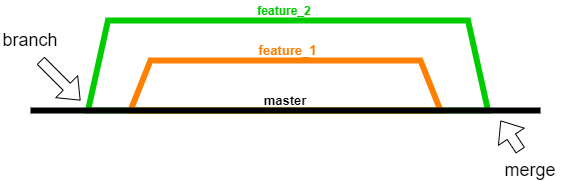
\includegraphics[width=1.0\textwidth]{./images/git_branching}
        \caption{Git Feature-Branch}
        \label{fig:gitbranching}
    \end{figure}
    A feature branch has two layers, first it has a master branch that contains the most up-to-date status of the
    project, containing all finalized features.
    Next to the master, many branches for the features that are currently being worked on exists.
    For every new feature, a branch is created.
    No work is ever done directly on the master, the master branch only contains fully finalised features.
    \begin{lstlisting}
		git checkout -b feature_1
    \end{lstlisting}
    \item \textbf{Add and commit} \\
    \begin{figure}[h]
        \centering
        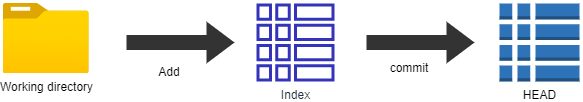
\includegraphics[width=0.8\textwidth]{./images/git_workflow}
        \caption{Git Workflow}
        \label{fig:gitworkflow}
    \end{figure} \\
    Git consists of three components in a tree.
    The first one is the Working directory, it holds all actual files of your current project.
    The second component of this tree is the index, also called \enquote{Staging Area}.
    Here you can decide what parts of the program should be taken into account for the next commit.
    The last component is called HEAD, it represents the local working repository of the current branch.
    If new files were created and you want to commit them, it is important to first add them to the index, so they are
    recognized during your commit to the HEAD. Every commit needs to have a commit message.
    Be wise and choose a message which shows which functionalities you added to the branch.
    \begin{lstlisting}
		git add <name of the file>
		git add *
		git commit -m "Commit Message"
    \end{lstlisting}
    \item \textbf{Push Changes} \\
    Right now, all changes are in the HEAD of the local repository.
    To send them to the remote repository run the following command:
    \begin{lstlisting}
		git push
		git push origin <branchname>
    \end{lstlisting}
    \item \textbf{Update} \\
    To update the local repository and getting the newest commits made to the remote repository run the command:
    \begin{lstlisting}
		git pull
		git pull origin <branchname>
    \end{lstlisting}
    The local repository is now merged with all changes from the remote repository.
    Doing a pull can result in merge conflicts.
    This happens for example, when there are differences in same part of the code between the local and the remote
    repository.
    Two avoid conflicts, all differences between two branches can be priviously be checked: \\
    \begin{lstlisting}
		git diff <branch1> <branch2>
    \end{lstlisting}

\end{enumerate}

\section{Integrated development environment (IDE)}\label{sec:integrated-development-environment-(ide)}

As integrated development environment (IDE) we had no given specification so everyone utilized their IDE of choice.
The utilized IDEs were mainly Visual Studio Code and PHPStorm by Jetbrains.

\section{Project Management Tools}\label{sec:project-management-tools}

For project management we utilized several tools.
For task tracking we focussed on Trello boards which provide several lists which can be named as preferred.
In our case we created a board with six different lists / columns:

\begin{itemize}
    \item TODO - tasks which are scheduled to be done in the project timeframe
    \item In Progress - tasks which are currently being worked on.
            This could be analysis or design tasks but also implementation.
    \item Review - tasks which are currently being reviewed or waiting for a review.
            This could be reviewing diagrams or code review on a pull request.
    \item Testing - tasks related to implementation which are not fully tested or where tests are not yet passing.
    \item In documentation - tasks which are functionality wise finished but still need to be documented
    \item Completed - tasks which are fully completed - no further action to be done.
\end{itemize}

We also made use of Visual Paradigm to create more complex diagrams such as a 
\textbf{\hyperref[sec:work-breakdown-structure-(wbs)]{work breakdown structure}}.

\section{Visual Design Tools}\label{sec:visual-design-tools}

For creating all sort of visual design related artefacts we utilized Adobe XD\@.
Adobe XD is a proprietary software offering a free plan to create user interface (UI) and user experience (UX)
related artefacts such as wireframes, design guidelines, grids as well as detailed designs.
